\documentclass[a4paper,12pt]{article} 
\usepackage[T1]{fontenc}              
\usepackage[frenchb]{babel} % césures, titres français
\usepackage[utf8]{inputenc} % encodage
\usepackage[a4paper,left=3cm,right=3cm,top=2cm,bottom=2cm]{geometry} % marges
\usepackage{graphicx} % insertion d'images
\usepackage{rotating}
\usepackage{float} % permet d'utiliser H pour placer un flottant obligatoirement
\usepackage{pdfpages} % inclusion de PDF au sein du document
\usepackage{listings}
\pagestyle{plain} % pied de pages simples

\setlength{\parskip}{1ex plus 0.5ex minus 0.2ex} % espace entre les paragraphes
\setcounter{tocdepth}{2}
\setcounter{secnumdepth}{2}

\lstset{% general command to set parameter(s)
basicstyle=\ttfamily, % print whole listing small
keywordstyle=\color{black}\bfseries\underbar,
% underlined bold black keywords
identifierstyle=, % nothing happens
commentstyle=\color{white}, % white comments
showstringspaces=false,
numbers=left,
language=java,
breaklines=true,
frame=tblr} % no special string spaces

%%%% debut macro %%%%
\makeatletter
\renewcommand\section{\@startsection {section}{1}{\z@}%
                           {-3.5ex \@plus -1ex \@minus -.2ex}%
                           {2.3ex \@plus.2ex}%
                           {\normalfont\Large\bfseries}}
\makeatother
%%%% fin macro %%%%



% Def
\newcommand{\code}[1]{{\lstinline{#1}}}

\begin{document}
\newpage
\title{TP Recherche d'Information}
\date{}
\author{BRIZAI Olivier\\THORAVAL Maxime}
\maketitle

\newpage
\section{Introduction}
Dans ce TP nous nous sommes intéressés à la mise en place d'une méthode d'indexation. La méthode d'indexation utilisée ici est fondée sur le facteur TF-IDF et le coefficient de Salton.

Le coefficicient TF-IDF permet de pondérer un mot dans le document auquel il appartient. Ce coefficient ne dépend pas seulement du nombre d'apparition du mot dans le document en question, mais également de
son apparition dans les autres documents. Une des propriétés remarquable de ce coefficient est donc justement de devenir très faible pour un mot donné, dans un index donné, si celui-ci est équi-réparti dans les documents de l'index. L'intérêt est alors de faire "disparaître" les mots très fréquemment utilisés dans les phrases comme ;  des pronoms personnels, conjonction de coordination, de subordination ...

Le coefficient de Salton permet quant à lui de classer les documents d'un index par pertinence lors d'une requête. Il se base pour cela sur une méthode dite vectorielle. L'objectif étant de calculer la "distance" d'une requête à chaque document de l'index et de classer ensuite les documents suivant cette distance. Le document le plus "proche" de la requête étant alors le plus pertinant. Plusieurs méthodes du calcul de cette distance sont envisageables.

\section{Choix de la structure}

Dans notre recdherche de la strcuture à utiliser, nous somme passés par plusieurs choix, et nous avons du revenir en arrière à plusieurs reprises.

Le premier choix était une structure de type : 

Hashmap< mot , Hashmap< document , pondération >  >

Lors de la phase d'indexation, ce choix est idéale puisque la complexité pour calculer la pondération TF-IDF est très bonne.
C'est au moment d'implémenter la phase de recherche dans l'index que nous sommes revenu sur cette structure. En effet avec une telle structure la complexité de la recherche dans l'index est très mauvaise.
Cela est du à la façon dont sont calculés les coeffcients de Salton.

La seconde structure que nous pouvions alors utiliser pour réduire le temps de recherche était : 

Hashmap< document , Hashmap< mot, pondération >  >

Cette solution réduit le temps de recherche mais c'est alors le temps d'indexation qui augmente.

Nous avons alors du faire un choix. Une possibilité aurait été de choisir les 2 structures à la fois. Cela aurait eu certes pour effet de doubler l'espace mémoire, mais on gagnait une puissance de N au niveau de la complexité.
Afin de ne pas trop nous écarter du sujet, nous avons donc tranché entre une des deux options et avons choisi la seconde. Notre choix a été orienté par la prise compte du fait qu'un utilisateur
ne doit pas attendre longtemps avant d'obtenir une réponse à sa requête. On pourra toujours lancer la phase d'indexation périodiquement. Dans la réalité les moteurs de recherche ne fonctionnent de toute façon pas de cette façon mais ce problème nous aura au moins fait prendre concience des problèmes à grande échelle.

\section{Améliorations et extensions}

Nous avons réalisé 4 améliorations du moteur d'indexation initialement écrit.

\subsection{Indexation des fichiers XML}

Dans la réalité un moteur de recherche va indexer tout type de document, qu'il s'agisse de document PDF, pages web (XML), fichiers texte, ...
Afin de donner cet aspect à notre moteur de recherche nous lui avons rajouté un parser de fichier XML. Nous pouvons donc désormais rajouter à l'index les mots d'un fichier XML, en plus de ceux des fichiers texte;

\subsection{Les Stop-Words}

Dans toute langue il existe un certain nombre de "mots" sur lesquels il est inutile de lancer une recherche. Il s'agit de mot "commun" à la langue et dont le sens est évident et inutile à préciser. Par exemple les lettres de l'alphabet ou des mots comme "le", "la", "les" ... Le but est donc ici d'agir lors de la phase l'indexation d'un document, en empêcheant celui-ci d'indexer ces "mots vides" (stop-word).

Pour cela nous avons nous sommes procuré une liste de "stop-word". Nous avons également rajouté une classe nommée "StopWordManager". Le StopWordManager est utilisé dans chaque parser de fichier. Une fois qu'un parser a récupéré tous les mots d'un document, ces derniers sont "filtrés" par le StopWordManager. Dans notre exemple, nous ne l'avons rajouté qu'au parser de fichier ".txt" mais on aurait très bien pu faire de même pour le parser de XML.

\subsection{Stockage de l'index}

\subsection{Pondération plus fine des mots d'une requête}

réaliser une pondération plus fine des mots d'une requête est une des améliorations que nous avons souhaité rajouter au moteur de recherche. Ceci a un sens si l'on
considère que l'utilisateur va mettre les mots qu'il considère comme les plus importants en premier. La première idée pour réaliser cela était de diminuer de façon linéaire le poids de chaque mot de la requête.
Mais un des inconvénients de cette méthode est qu'au bout d'un certain nombre mots, les mots restants auront un poids nul et ne compteront donc plus dans le requete. Si mot est présent dans la requête mais que tous les mots qui le précèdent n'apparaissent pas dans les recherches, ce dernier mot a tout de même droit à sa chance.

Pour remédier à cela on a utilisé une fonction qui converge vers 0 à l'infini. Ainsi le coefficient décroit en permanence sans atteindre zéro (sauf arrondissement inévitable au bout d'un certain temps).
mais cette fonction a également un autre intéret. Doit-on en effet considérer que le passage du 1er au 2nd mot est aussi important que le passage du 7ème au 8ème mot dans la recherche ? Nous avons pensé qu'il pouvait-être
intéressant de donner plus de poids aux premiers mots (les trois premiers par exemple) mais que les poids des mots suivants décroissent plus rapidement. On a donc cherché une fonction qui décroisse doucement au début puis accélère ensuite.

Au final nous avons utilisé la fonction : \[\exp(-(\frac{x}{5})^{2})\]

On obtient alors les pondération 1, 0.96, 0.85, 0.70, 0.53

\begin{figure}[H]
	\center
	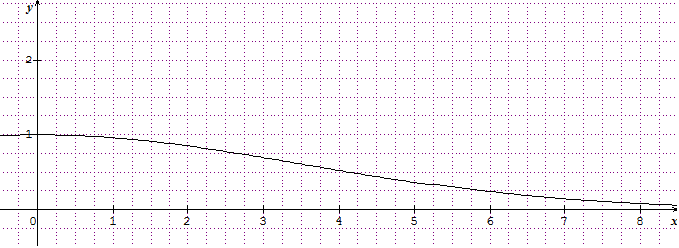
\includegraphics{courbe.png}
	\caption{Courbe représentative de la fonction utilisée pour pondérer les requêtes}
\end{figure}

Bien sur cette fonction n'est là que pour illustrer la démarche générale de cette pondération plus fine et n'est pas forcément la plus optimale à utiliser.

\section{Bilan du TP}

L'objectif de ce TP n'était pas de réaliser le plus performant des moteur de recherche ni d'utiliser la meilleur méthode d'indexation. A travers cet exemple nous avons pu découvir différentes notions
que toute personne travaillant dans ce domaine doit garder à l'esprit. Lorsque l'on traite une quantité d'information gigantesque, on ne traite pas l'information de la même manière car le mondre coût suplémentaire
aura un impact énorme.
\end{document}


